\chapter{Related Works}
\label{chp:relworks}


In this chapter, we give a description of previous works related to this thesis. Spatial alarm processing technique in Road Network and Euclidean Space has been extensively studied in recent years.In this chapter, we first show the related works on Spatial Alarm queries in Road Networks in Section~\ref{sec:NN}, Group nearest neighbor (GNN) queries in Obstructed Space in Section~\ref{sec:ANN} Efficient Spatial Alarm finding techinques in Section~\ref{sec:GNN}, and finally a discussion on R-tree as an efficient data structure for indexing spatial alarms is given in Section ~\ref{sec:R}.


Extensive research has been performed and various  effective algorithms have been proposed \cite{roadalarm},\cite{mur},\cite{bamba} to process spatial alarms in Euclidean space and road network in recent years. Euclidean space considers the straight line distance between two points irrespective of obstacles on the other hand in road networks navigation is limited along predefined roads.\\ Obstructed space considers the shortest distance between two points in the presence of obstacles. Various spatial range query algorithms have been presented in recent times \cite{obst1},\cite{obst2},\cite{ognn} such as nearest neighbour and group nearest neighbour in obstructed space.\\
Again, comprehensive research \cite{liu} has been conducted to make spatial alarm evaluation energy-efficient and effective in road networks. 
However, to the best of our knowledge no research work has yet been published on the topic of spatial alarms in obstructed space.

\section{\label{sec:NN}Road Alarm}
NN queries  and $k$ nearest neighbor ($k$NN) queries constitute a very important category of queries in database studies. They have many kinds of applications including but not limited to geographic information systems GIS, CAD/CAM, multimedia ~\cite{AP1}, knowledge discovery~\cite{AP2} and data mining. The first problem of answering $k$NN queries using the R-tree was first introduced in~\cite{NN1}. That algorithm searches the R-tree in a depth first manner, using two different metrics to help pruning intermediate nodes and leaf nodes. One metric is optimistic mindist, which corresponds to the shortest distance between the query point and the MBR (Minimum Bounding Rectangle) of a tree entry. The other is pessimistic minmaxdist, which measures the longest distance from the query point to a tree entry MBR that ensures the existence of some data point ($s$). For a given query point $q$, mindist and minmaxdist are used to order and prune R-tree node entries according to three heuristics:


\begin{itemize}
\item  Every MBR M with mindist ($q$,M) greater than the actual distance from $q$ to a given object $o$ is discarded;
\item For two MBRs M and M', if mindist ($q$,M) is greater than minmaxdist ($q$,M'), M is pruned;
\item  If the distance from q to a given object o is greater than minmaxdist ($q$,M) for an MBR M, $o$ is discarded.
\end{itemize}

The depth-first $k$NN algorithm accesses more R-tree nodes than necessary. To enable optimal index node access, a best-first algorithm was proposed in~\cite{NN2,NN3}. A memory heap is used to hold the R-tree entries to be searched, which gives priority
to smaller mindist between an entry and the query point. Entries for the memory heap are selected according to the mindist between an entry and the query point. Only those entries with a small enough mindist are pushed into the heap and searched later with its sub-entries checked and pushed back if necessary. With the optimization done with the metric mindist, the best-first algorithm only accesses those nodes containing $k$ nearest neighbors, thus achieving optimal node access.

Yu et al.~\cite{NN5} proposed an efficient method, called iDistance, for $k$ nearest neighbor $k$NN search in a high-dimensional space. iDistance partitions the data and selects a reference point for each partition. The data in each cluster are transformed into a single dimensional space based on their similarity with respect to a reference point. This allows the points to be indexed using a B+-tree structure and $k$NN search be performed using one dimensional range search. The choice of partition and reference point provides the iDistance technique with degrees of freedom most other techniques do not have. They describe how appropriate choices here can effectively adapt the index structure to the data distribution.

The majority of the research before~\cite{NN6} were based on Euclidean distance between the points. The first contribution of this paper is that it demonstrates Euclidean metric is not good distance approximation for road network. In that case they worked with real-world dataset. And they conclude that about 40\% false hits are counted when Euclidean distance is used.

Shekhar et al.~\cite{NN7} introduced In-route nearest neighbor query, called IRNN. They discussed four different techniques namely Simple Graph-Based (SGB), Recursive Spatial Range query-based (RSR), Spatial Distance Join-based (SDJ) and Precomputed Zone-based
(PCZ) solution. Precomputed zone-based method always outperforms the other methods when there are no updates on the road map. However, the response time of the precomputed zone-based method dramatically increases with increases in the update ratio I/Os. It also needs more storage space for storing the Precomputed results. In the other methods, the overall response time decreases with increases in the facility density and increases with increases in the route length and the size of the road map. The spatial distance join-based method outperforms the recursive methods with fewer numbers of path computations. The experiment shows that the strategy to reduce the number of path computations to minimize the response time is reasonable. However, in the dense road map area, the performance of the recursive spatial range query-based method declines due to the increase of the false hit ratio of the Euclidean candidates and the simple graph-based method shows better response time than the spatial range query-based method.

Conventional NN search (i.e., point queries) and its variations in low and high dimensional spaces have received considerable attention (e.g.~\cite{NN9, NN4} due to their applicability in domains such as content based retrieval and similarity search. Because of the proliferation of location based e-commerce and mobile computing, continuous nearest neighbor CNN search promises to gain similar importance in the research applications communities. Algorithm of CNN query first introcuced in~\cite{NN10} in which  the proposed solution has the false misses and the high processing cost. In~\cite{NN4} the study of the problem is done
extensively and propose algorithms that avoid the pitfalls of previous ones, namely, the false misses and the high processing cost. They also propose theoretical bounds for the performance of CNN algorithms and experimentally verify that their proposed methods are nearly optimal in terms of node accesses.

However Kolahdouzan and Shahabi~\cite{NN11} introduced Voronoi-Based  $k$ Nearest Neighbor Search for Spatial
Network Databases.

\section{\label{sec:ANN}Energy Efficient Middle Ware Architecture for processing spatial alarms on Mobile Clients}
Papadias et al.~\cite{ANN1} have proposed and solved query processing in the context of large road network by extending $k$NN queries. They proposed three algorithms that solve ANN queries by effectively minimizing network traversal. The first one utilizes Euclidean lower bounds and an incremental Euclidean ANN method. The other two algorithms are motivated by aggregate top-k query processing techniques. The incremental Euclidean restriction IER incrementally retrieves Euclidean aggregate nearest neighbors and computes their network distances by shortest path queries until the result cannot be improved. TA and CE explore the network around the query points until the aggregate nearest neighbors are discovered. Their techniques can be applied for various aggregate distance functions (sum and max). In addition, they can be combined with spatial access methods and shortest path materialization techniques. A thorough experimental study suggests that their relative performance depends on the problem characteristics. IER is the best algorithm when the edge weights are proportional to their lengths since, in that case, Euclidean distance becomes a quite tight lower bound of the actual network distance. Nevertheless, the performance of IER degrades fast as the weights are less reflected by the edge lengths. For such cases, threshold algorithm TA is the most appropriate method for sum queries, whereas CE concurrent expansion  is the best approach for max queries. In addition, TA and CE are the only choices when the interesting points are not indexed by R-trees or when the Euclidean distance bounds may not be used (e.g., in non spatial networks).


\section{\label{sec:GNN}Group Nearest Neighbor Queries in Obstucted Space}
A group nearest neighbor (GNN) query~\cite{gnn:papa,GNN1,GNN2} is slightly different form of NN query, finds the nearest data point with respect to all user locations of a particular group. A GNN query minimizes the aggregate distance for the group, where an aggregate distance is computed as the total, minimum or maximum distance of the data point from the group. Papadias et al.~\cite{gnn:papa} have proposed three techniques: multiple query method MQM, single point method SPM, and minimum bounding method MBM, to evaluate GNN queries.


\begin{itemize}
\item The multiple query method MQM is a threshold algorithm. It executes incremental NN search for each point $q_{i}$ in Q, and combines their results. The distance to $q_{i}$'s current NN is kept as a threshold $t_{i}$ for each $q_{i}$. The sum of all thresholds is used as the total threshold T. best dist is dist ($NN_{cur}$, Q), where $NN_{cur}$ is the candidate nearest neighbor found so far. Initially, best dist is set to 1 and T is set to 0. The algorithm computes the nearest neighbor for each query point incrementally, updating the thresholds and best dist until threshold T is larger than best dist.

\item The single point method SPM processes a GNN query in a single traversal of the R-tree. SPM first decides the centroid $q$ of Q, which is a point in the data space with a small or minimum value of dist ($q$, Q). Then a depth-first $k$NN as the query point. During the search, some heuristics based on triangular inequality is used to prune intermediate nodes and determine the real nearest neighbors to Q.

\item The minimum bounding method MBM regards Q as a whole and uses its MBR M to prune the search space in a single query, in either a depth-first or best-first manner. Two pruning heuristics involving the distance from an intermediate node N to M or query points are proposed and can be used in either manner.
\end{itemize}


If we compare among the above three techniques MQM retrieves the NN for every point in query set Q, it sometimes accesses the same tree nodes more than once for different query points, so it causes the overhead while high query set cardinality is adopted. In contrast with MQM, both SPM and MBM perform a single query with some pruning heuristics. SPM is a modified single depth-first $NN$ search with the centroid of Q being the query point while MBM considers the MBR of Q with best-first manner. The distribution shape of query points in Q has an impact on the performance of SPM and MBM because the former approximates $q_{i}$'s centroid and uses it in the single query, and the latter takes into account the extent of Q when pruning nodes. According to the comparison conducted in ~\cite{gnn:papa} among these three techniques, MBM performs the best as it traverses the R-tree once and takes the area covering the user's location into consideration.

Li et al.~\cite{geq:p} have showed the MBM method only inspects the triangle inequality and there all other important pruning and optimization opportunities are failed to achieve. That is why they introduced a heuristic approach having query cost $O(N+M)$ according to the assumed facts. They first addressed a new exact method which has much lower query cost in compare to MBM method. They also explore high-quality approximation method that is bounded to logarithmic query cost and it has approximation ratio $\sqrt{2}$ in the worst case for a fixed dimension.

Huang et al.~\cite{pgnn:s} have evolved two pruning strategies namely distance pruning method and MBR pruning method for GNN queries over spatial datasets indexed by the R-tree. By taking into account the distribution of all query points, we use an ellipse in both methods to approximate the query extent. Then a distance or MBR derived from the ellipse is used to prune intermediate index nodes during search. The proposed pruning strategies can be used in both the depth-first and best-first traversal paradigms. The experimental results demonstrate that their proposed methods outperform the existing ones significantly and consistently with real geographical datasets, in both page access number and CPU time.





\section{\label{sec:GTPQ}Group Trip Planning Queries}
Location-based social networks such as Facebook~\cite{facebook}, Google+~\cite{google}, and Loopt~\cite{loopt} have enabled a group of friends to remain connected virtually from anywhere at any time via location aware mobile devices. In this regard, GTP query problem~\cite{Tanzima:Ali} has been introduced for multiple sources and destination locations in Euclidean distance. In that purpose they presented two algorithms, among them one is iterative method as baseline algorithm and the other is an efficient hierarchical method. The iterative algorithm does not evaluate the trip planning query individually for every user but still have to access the same database more than once that causes more queries processing overhead. And on the other hand they evolved hierarchical algorithm that evaluates $k$-GTP queries with a single visit to the database and renders less processing overhead. They proposed hierarchical algorithm based on two heuristics, GTP-HA1 and GTP-HA2. Heuristic 1 and heuristic 2 are yielded to compute smaller upper bound of total distance. In terms of I/Os if the three algorithms are compared, iterative algorithm requires two orders of magnitude more I/Os than that of hierarchical algorithm. And GTP-HA1 takes on average 20\% more I/Os and 27\% more processing time than GTP-HA2.


In general when the users plan a trip that includes different types of data objects the number of different data points is typically restricted to 2 or 3. For example a group would like first go for shopping, taking dinner afterwards and possibly go to watch cinema later on. When a group will be planned for a large number of places   and considered for flexible k-GTP queries then the query processing time may cause higher complexity. Let consider a group specify the order of visiting types \{2,1,3\} then in case of flexible group they also have to compute \{3,1,2\},\{1,2,3\}, \{3,2,1\},\{1,3,2\},\{2,3,1\}. So m$>$1 we have to consider m! visiting types for computing k-GTP queries. Thus they set the number of data types (m) to 2 and 3. They also provide the reason to consider ordered k-GTP queries because of a group wants to visit different places they know beforehand in which order they will visit the different places.

\section{\label{sec:R}R-Tree: An efficient indexing Method}
\begin {figure}[htbp]
\centering
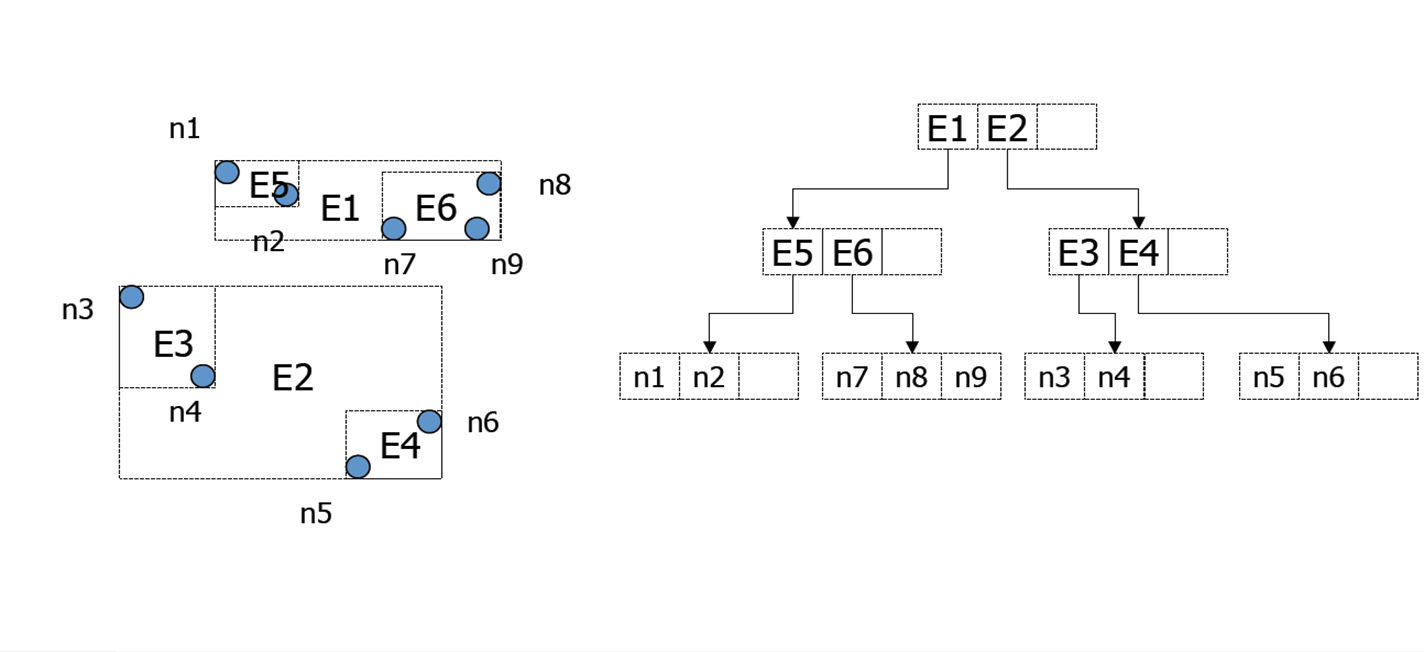
\includegraphics [width= 150mm]{figures/rtree.png}
\caption{MBR corresponding to a R-tree}
\label {overflow}
\end{figure}
B-tree~\cite{BTREE} is a data structure for storing data with amortized run times for insertion and deletion in logarithmic time. It is often used for data storing on long latency I/Os (such as file systems and Data bases) because child nodes can be accessed together since they are in order. B-tree can not store new type of data (i.e. geometrical data, multi-dimensional data). So Guttman ~\cite{RT2} provided R-Tree to do that. R-tree~\cite{RT3,RT4} has some variants and the following properties in common-
\begin{itemize}
\item  R-Trees can organize any-dimensional data by representing the data by a minimum bounding rectangle MBR.
\item Each node bounds it's children. A node can have many objects in it.
\item The leaves point to the actual objects which are stored on the disk.
\item The height is always log n (It is height balanced).

\end{itemize}


\endinput 